This section introduces basic \LaTeX\ syntax. Learn how to configure the project Preamble then write your first section in \LaTeX\ code!
\subsection{Basic LaTeX}
Authoring with \LaTeX\ is similar to writing a program: type code to define program behavior, compile program into consumable file, then open file and enjoy! There are four key principles to consider when authoring documents with \LaTeX:
\begin{enumerate}
    \item Content is written in plaintext.
    \item Formatting and features are applied with commands.
    \item Packages provide extra text, graphics, and presentation commands.
    \item \LaTeX code is typically compiled into a read-only professional-looking PDF.
\end{enumerate}
With these principles in mind, let's start learning some basic \LaTeX\ syntax and commands\footnote{Based on existing instructional material: http://www.rpi.edu/dept/arc/training/latex/class-slides-pc.pdf}.
%TODO: Cite this
\par
The \verb|"\"| backslash character is used to begin all \LaTeX\ commands. E.g.
\verb|\LaTeX| compiles to \LaTeX.
\par
Some commands take input enclosed in curly braces. E.g.
\verb|\textit{}{Some italicized text}| compiles to \textit{Some italicized text}.
\par
{\Large\textbf{Common commands include:}\\}
\verb|\\|, \verb|\newline|, \verb|\par|\\
Various ways to generate new lines.
\par
\verb|\newpage|\\
Insert page break to start text on new page.
\par
\verb|\textit{text}|, \verb|\textbf{text}|, \verb|\texttt{text}|\\
Modifies text to be \textit{italicized}, \textbf{bold}, or \texttt{scientific}.
\par
\verb|\usepackage{<packageName>}|\\
Define a \LaTeX\ package to use for modular commands and behaviors in your project.
\par
\verb|\chapter{<title>}|, \verb|\section{<title>}|, \verb|\subsection{<title>}|\\
Mark the beginning of new chapters/sections/subsections.
\par
\verb|\begin{document}| and \verb|\end{document}|\\
Define area for all the text of the document.
\par
\verb|\begin{abstract}| and \verb|\end{abstract}|\\
Define area for the abstract of the document.
\par
\verb|\title{<document title>}|, \verb|\author{<author>}|, \verb|\date{<date>}|\\
Define the document's title, author, and date.
\par
\verb|\maketitle|\\
Print the document's title, author, and date.
\par
\verb|\markboth{left title}{right title}|\\
Defines the headings or footings on either side of the page.
\par
{\Large\textbf{Certain characters have special meanings in \LaTeX.}}
\par
\begin{tabular}{r|l}
\textbf{Char} & \textbf{Meaning} \\
\verb|%|& Parameter in a macro; also used in tables \\ 
\verb|$|& Used to begin and end math mode \\
\verb|%|& Used for comments in the source file \\
\verb|&|& Tab mark, used in alignments and tables \\
\end{tabular}
\par
See comprehensive guide about \LaTeX\ commands and characters at \url{http://www.rpi.edu/dept/arc/docs/latex/latex-intro.pdf}. In the next subsection, you will use basic knowledge of \LaTeX\ to configure the Preamble of your project.

\subsection{The Preamble}
We previously set the \texttt{Main Document} of the project in Overleaf to
\path{layout_e.tex}. Locate this file and open it to begin adding content to your project.

\begin{minipage}{\linewidth}
\centering
\fbox{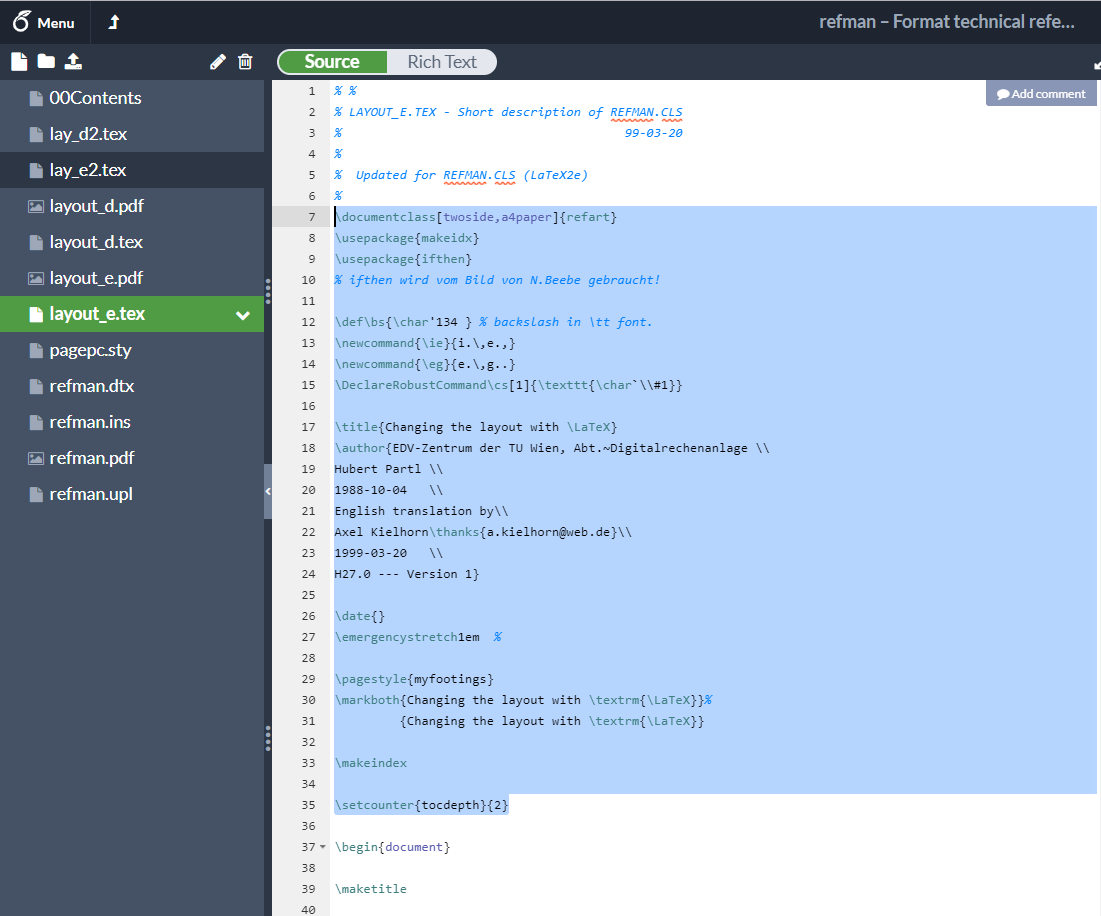
\includegraphics[width=\linewidth]{graphics/MainDocumentPreamble.PNG}}
\captionof{figure}{Locating \detokenize{layout_e.tex file}}
\label{fig:Preamble}
\end{minipage}

Notice the highlighted section in figure \ref{fig:Preamble}. The area of from the start of the document to the \verb|\begin{document}| command is the \texttt{Preamble}: the first part a file where you describe \LaTeX\ document type, commands, and more information about the document.

We will configure the Title, Author, Date, Packages Used, and Formatting of the \LaTeX\ document in he Preamble using \LaTeX\ syntax and commands.

\subsubsection{}
To begin configuring the \texttt{preamble}, extend the available features in your \LaTeX\ project by adding the following commands after \verb|\usepackage{ifthen}|.
\begin{verbatim}
\usepackage{url}
\usepackage{csquotes}
\usepackage{graphicx}
\usepackage{float}
\usepackage{caption}
\usepackage{hyperref}
\usepackage{titlesec}
\usepackage{todonotes}
\usepackage{subcaption}
\usepackage{xcolor}
\usepackage{nameref}
\usepackage{listings}
\usepackage{verbatim}
\usepackage[T1]{fontenc}
\end{verbatim}

\subsection{Modifying Section}